\chapter{Architektura oprogramowania i zaplecze aplikacji}
\label{chap:ZapleczeAplikacji}
\textit{Autor: Piotr Noga}
\par Niemniej ważnym elementem naszej pracy, od przedstawionej w rozdziale \nameref{chap:InterfejsGraficznyUżytkownika} warstwy prezentacji danych, było zaimplementowanie systemu, który byłby odpowiedzialny za przechowywanie wszelkich danych, które są wykorzystywane w trakcie działania aplikacji oraz za logikę biznesową, umożliwiającą działanie algorytmów zaprezentowanych w rozdziale \nameref{sec:POSUzycie} czy też odpowiednie przetwarzanie informacji między użytkownikiem a wspomnianą wcześniej warstwą przechowywania danych.
Tę sekcję aplikacji przyjęło się w nomenklaturze informatycznej nazywać zapleczem.

\section{Architektura oprogramowania}
\label{sec:ArchitekturaOprogramowania}
Przed opisem zaplecza należy się zagłębić nad architekturą oprogramowania, gdyż to od niej tak naprawdę zależy, jak zostanie on zaimplementowany. Architektura ta wskazuje m.in. potrzeby jakie ma spełniać program oraz w jaki sposób powinien je realizować \cite{AO}.

\subsection{Architektura rozproszona}
\label{sec:Rozproszenie}
Jednym z założeń w naszej pracy jest zastosowanie architektury rozproszonej. Celem tego założenia jest to, aby można było zapisywać dane w taki sposób, żeby nie były one przechowywane tylko w jednym miejscu, gdyż mogłoby to doprowadzić do ich utraty, chociażby w przypadku awarii systemu. Taką potrzebę można spełnić poprzez zapisywanie danych, które są dystrybuowane na inne komputery poprzez sieć P2P. 
\begin{figure}[!ht]
	\centering
		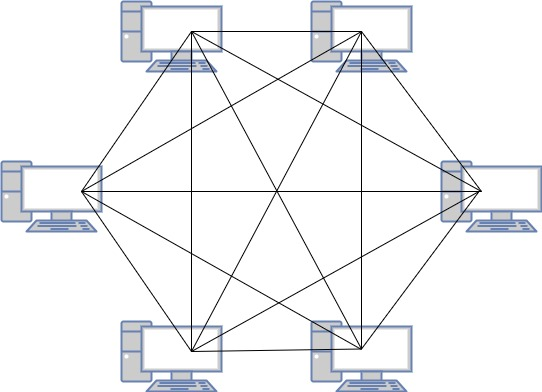
\includegraphics[width=0.3\textwidth]{Images/P2P.jpg}
	\caption{Sieć typu P2P}
	\label{fig:P2P}
\end{figure}
\newline Każdy z komputerów połączonych do takiej sieci zawierałyby swoją własną kopię danych, dzięki czemu przy utracie danych na którymś z komputerów, można je odzyskać poprzez pobranie ich od innego użytkownika.
Istnieje również alternatywne rozwiązanie tego założenia, mianowicie przechowywanie danych na różnych serwerach. Jest to w obecnych czasach częściej spotykane rozwiązanie, lecz nie spełnia ono kolejnej potrzeby, która jest opisana w następnej sekcji.
\begin{figure}[!ht]
	\centering
		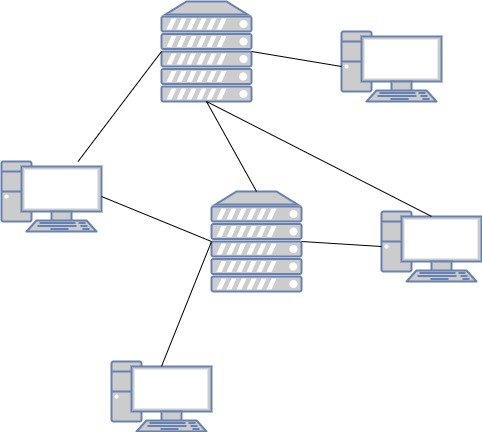
\includegraphics[width=0.3\textwidth]{Images/Siec_serwery.jpg}
	\caption{Sieć z różnymi serwerami}
	\label{fig:SiecSerwery}
\end{figure}
\newline

\subsection{Decentralizacja}
\label{sec:Decentralizacja}
Kolejnym wymogiem, jaki powinien być zrealizowany w naszej pracy, jest wykonanie aplikacji, która będzie działać w sposób zdecentralizowany. Oznacza to, że żaden użytkownik nie może mieć kontroli nad innymi, a co za tym idzie, nie ma żadnej scentralizowanej jednostki, która może zarządzać przepływem danych w sieci. Z tego powodu drugie rozwiązanie, które zostało wspomniane w poprzedniej sekcji, czyli wykorzystanie różnych serwerów do przechowywania danych, nie może zostać wykorzystane w naszej implementacji. Wynika to z faktu, iż osoby zarządzające serwerami mogą arbitralnie zablokować niepożądanym w ich ocenie osobom dostęp do zasobów danych.


\section{Logika biznesowa}
\label{sec:LogikaBiznesowa}
Należy na początku poświęcić kilka słów wyjaśnienia, co kryje się pod pojęciem logika biznesowa. Jest to warstwa aplikacji odpowiedzialna za wykonywanie funkcji, które umożliwiają jej prawidłowe oraz spójne działanie. Kontroluje ona, co użytkownik może wykonać w aplikacji oraz definiuje warunki, jakie muszą zajść, by do danej czynności doszło. Przykładowo użytkownik może w programie definiować nowe zadanie, lecz jest to obarczone konkretnymi warunkami, takimi jak: 
\begin{itemize}
    \item projekt, w którym chce je dodać, musi istnieć,
    \item użytkownik musi mieć do dostęp do tego projektu,
    \item musi uzupełnić szczegóły dotyczące nowego zadania jak chociażby nazwa zadania czy też jaka osoba jest do niego przypisana.
\end{itemize}
Niespełnienie któregokolwiek z warunków sprawia, że nie może zostać utworzone nowe zadanie. Logika biznesowa nie zajmuje się wyłącznie tym, gdyż wykonywane są w niej również wspomniane na początku rozdziału algorytmy. Implementacja ich w tym miejscu związana jest z co najmniej z dwoma potrzebami, które należy spełnić w naszym programie, mianowicie są to:
\begin{itemize}
    \item możliwie jak najkrótszy czas dostępu do danych,
    \item responsywność interfejsu graficznego.
\end{itemize}
Dostęp do danych powinien jak najwierniej odwzorowywać operacje atomowe na mikroprocesorze, tak aby był on możliwie najkrótszy. To sprawia, że gdy przykładowo inny użytkownik będzie chciał pobrać od nas jakieś informacje, to żeby nie musiał oczekiwać na zwolnienie zasobu, który jest wykorzystywany do wyliczania wyniku algorytmu. W warunkach, w których przeważnie testowaliśmy nasz program, czyli uruchomionych kilka klientów, nie byłoby odczuwalnej różnicy w czasie dostępu, natomiast jeśli przełożyć tę różnicę na chociażby kilkaset klientów, to każda próba pobrania od innych użytkowników danych wiązałaby się ze zwiększonym opóźnieniem. Podobnie jak do czasu dostępu rzecz ma się z responsywnością interfejsu, gdyż gdyby on musiał wykonywać obliczenia związane z algorytmami, to użytkownik mógłby odczuć, jakby program co chwila nie odpowiadał.
%--TODO--

\subsection{Komunikacja między użytkownikami}
\label{sec:Komunikacja}
Jednym z istotnych elementów naszego programu jest możliwość komunikowania się ze sobą użytkowników. W tym celu wykorzystaliśmy porozumiewanie się za pomocą protokołu HTTP. Wynika to z następujących zapotrzebowań:
\begin{itemize}
    \item bezpośrednia komunikacja między użytkownikami,
    \item dostosowanie przesyłanych danych w zależności od kontekstu,
    \item prostota zastosowania danego protokołu,
    \item szeroko dostępna dokumentacja protokołu.
\end{itemize}
Alternatywą do HTTP jest IPFS - InterPlanetary File System, który na pierwszy rzut oka wygląda na  lepsze rozwiązanie do naszej pracy, gdyż w przeciwieństwie do HTTP jest przystosowany do pracy w sieci rozproszonej, czym jest głównie reklamowany \cite{IPFS}. Nie wybraliśmy go jednak w naszej pracy ze względu na wcześniejsze doświadczenie z protokołem HTTP w poprzednich naszych projektach oraz na znikomą ilość pomocy dydaktycznej związanej z wykorzystaniem go w aplikacjach. Problemem z IPFS jest również to, że jego przystosowanie do sieci rozproszonej tyczy się treści przesyłanych przez ten protokół, aniżeli komunikacji między osobami. Jest to dobre rozwiązanie w przypadku, gdyby nasza aplikacja polegała wyłącznie na przechowywaniu danych i przesyłaniu ich między użytkownikami. Ze względu na zastosowanie łańcucha bloków, o którym można więcej przeczytać w sekcji \nameref{sec:Blockchain}, w którym zapisywanie danych nie odbywa się natychmiast, nie jest to koniecznie dobre rozwiązanie.
\clearpage
\begin{figure}[!ht]
    \centering
		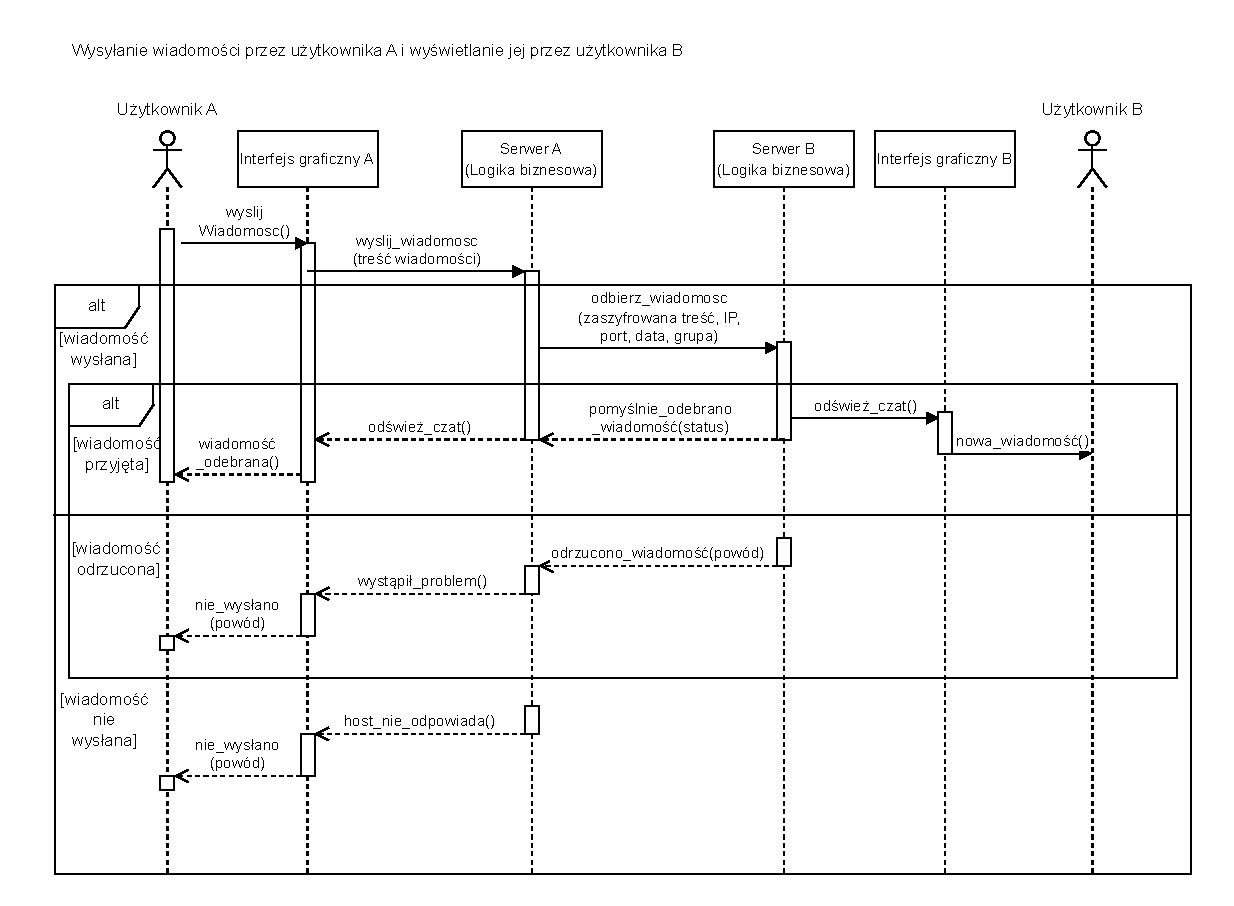
\includegraphics[width=1\linewidth]{Images/wysylanie_wiadomosci.pdf}
	\caption{Diagram sekwencji wysłania wiadomości i jej wyświetlenia}
	\label{fig:wysylanieWiadomosci}
\end{figure}
\par Po przedstawieniu cech protokołu HTTP i uzasadnieniu jego wyboru, pora przejść do omówienia tego, jak on jest w praktyce wykorzystywany w naszej pracy. Komunikacja po tym protokole dostępna jest za sprawą uruchamianego w naszym programie serwera. Odpowiedzialna jest za to biblioteka dostępna w języku Python - \textit{Flask}. Umożliwia on otrzymywanie danych od innych użytkowników jak również odsyłanie im odpowiedzi wraz z żądanymi informacjami. Diagram sekwencji przedstawiony w \figurename{ \ref{fig:wysylanieWiadomosci}} posłuży tutaj jako ilustracja przykładu takiej komunikacji. Sytuacja na tym diagramie jest następująca: Użytkownik A pragnie wysłać wiadomość do Użytkownika B, a ten chce wyświetlić jej treść. W celu uproszczenia diagramu zakładamy, że obaj użytkownicy mają otwarty czat ze sobą, zatem interfejs graficzny nie przesyła informacji, jakiego czatu dotyczą dane wiadomości. Na początek Użytkownik A wypełnia w interfejsie graficznym aplikacji pole wiadomości jej treścią i zleca programowi jej wysłanie. Warstwa prezentacji przesyła odpowiednie informacje do logiki biznesowej aplikacji, tj. treść wiadomości. Następnie logika biznesowa w ramach bezpieczeństwa szyfruje wiadomość kluczem prywatnym Użytkownika A. W tym momencie następuje komunikacja między użytkownikami za pomocą protokołu HTTP, gdyż logika biznesowa zleca serwerowi, uruchomionemu w oddzielnym wątku, wysłanie zapytania HTTP do serwera Użytkownika B pod odpowiedni adres. Struktura adresu wygląda następująco:
\begin{lstlisting}[caption={Struktura adresu docelowego}]
http://<Adres IP>:<Numer portu>/<funkcja_do_wywolania>
\end{lstlisting}
W tym konkretnym przypadku przedstawionym na diagramie, w naszym projekcie byłby to adres
\begin{lstlisting}[caption={Adres docelowy wywołania funkcji odbierania wiadomości}]
http://<Adres IP>:<Numer portu>/receive_message
\end{lstlisting}
Wysłanie żądania odbywa się za pomocą gotowej funkcji przygotowanej w bibliotece \textit{Flask}, odpowiedzialnej za działanie serwera (funkcja \textit{requests.post()}). Wszelkie dane, które mają trafić do drugiej osoby, zapisywane są w formacie JSON. Po wysłaniu zapytania HTTP, serwer Użytkownika B odbiera je i przekazuje dalej do logiki biznesowej. W przypadku, gdy Użytkownik B otrzymał prawidłową wiadomość, wysyła odpowiedź HTTP ze statusem sukcesu, oznaczającym wysłanie prawidłowego żądania. Jeśli jednak z jakiegoś powodu Użytkownik A wysłał błędną wiadomość, np. została źle sformatowana, bądź Użytkownik B posiada przestarzały klucz publiczny wysyłającego, przez co nie mógł jej prawidłowo odszyfrować, to wysyła odpowiedź ze statusem błędu. Użytkownik A w zależności od tego, jaką otrzymał odpowiedź, wykonuje odpowiednią czynność. Dodaje on do swojej puli wiadomości tę wysłaną do Użytkownika B tylko wtedy, gdy się okaże, że została ona prawidłowo odebrana. Zostało to również odzwierciedlone na analizowanym diagramie.

\section{Przechowywanie danych}
\label{sec:PrzechowywanieDanych}
Trzecią z warstw aplikacji, jakie można wyodrębnić zaraz po warstwie prezentacji (interfejsu graficznego) oraz logiki biznesowej, jest warstwa przechowywania danych. Jest ona odpowiedzialna za dostęp do danych używanych w trakcie korzystania aplikacji. Warstwa ta ma gwarantować to, że w możliwie jak najkrótszym czasie uzyska się żądane dane oraz ich zapis przebiegnie bez najmniejszych zakłóceń. W przypadku awarii systemu i utraty danych z tego tytułu, warstwa ta powinna być w stanie odtworzyć je na podstawie ich kopii, które znajdują się na komputerach innych użytkowników. Proces ten powinien przebiegać na tyle sprawnie, żeby użytkownik mógł nawet nie zwrócić uwagi na fakt, że przez krótki czas mógł mieć błędne dane.
%TODO

\subsection{Łańcuch bloków}
\label{sec:Blockchain}
Użycie sieci P2P w naszej pracy sprzyja temu, by skorzystać ze struktury danych, która jest przystosowana do takiego rozwiązania. Jedną z takich struktur jest łańcuch bloków \ang{Blockchain}. Jest to jednokierunkowa lista, w której nowe rekordy, zwane blokiem, są przyłączane zawsze na jej końcu. Każdy z tych bloków jest odpowiednio przywiązany do ich sąsiadów. Jest to możliwe dzięki zastosowaniu odpowiednio zaszyfrowanego skrótu z treści \ang{Hash} poprzedzającego go bloku. Przywiązanie te najprościej będzie przedstawić na podstawie naszego kodu, w którym widoczne są pola, jakie zawiera obiekt klasy Block.
\begin{lstlisting}[language=Python, extendedchars=true, caption={Pola obiektu klasy Block}]
self.index
self.data
self.digitalEncryption
self.hostVerifier
self.portVerifier
self.publicKeyVerifier
self.lastDigitalEncryption
\end{lstlisting}
Pola tej klasy służące do łączenia ze sobą bloków to \textit{digitalEncryption} oraz \textit{lastDigitalEncryption}, z czego to pierwsze informuje o skrócie z treści aktualnego bloku, a drugie z bloku poprzedzającego. Przy tworzeniu łańcucha bloków należy stworzyć również blok "zerowy". Wynika to z faktu, że pierwszy blok, który rozpoczyna łańcuch, nie posiada swojego poprzednika, zatem pole \textit{lastDigitalEncryption} musi mieć ustawioną specjalną wartość. W różnych implementacjach łańcucha bloków, jakie napotkaliśmy w publicznych repozytoriach kodów jak np. \url{https://github.com} najczęściej spotykaliśmy rozwiązanie, że skrót treści "zerowego" bloku był przepisywany do pola z  wartością poprzednika. Z takiego pomysłu również skorzystaliśmy w naszej implementacji łańcucha bloków, którą bazujemy na implementacji znajdującej się w repozytorium pod linkiem: \url{https://github.com/breqdev/blockchat} (Dostęp: 2024-12-07). Poza tymi dwoma polami, warto zwrócić uwagę również na pozostałe. Pole \textit{index} umożliwia pozycjonowanie bloków w całym łańcuchu, natomiast pole \textit{data} jest tym kluczowym, gdyż właśnie w nim zapisywane są wszelkie dane odnośnie grupy wiadomości czy informacji na temat sfinalizowanego projektu z modułu planera. Grupa wiadomości to nic innego jak zbiór \textit{x} wiadomości przesłanych między użytkownikami, gdzie \textit{x} oznacza ich liczbę. Domyślnie jest to wartość 20. Pola \textit{hostVerifier}, \textit{portVerifier} oraz \textit{publicKeyVerifier} są związane ze szyfrowaniem bloku przez podpis odpowiedniego sygnatariusza, czyli osoby wybranej w PoS do zweryfikowania autentyczności otrzymanych danych. Te pola to odpowiednio: adres IP, numer portu oraz klucz publiczny tego użytkownika. Więcej informacji odnośnie roli tej osoby przy szyfrowaniu bloku znajduje się w rozdziale \nameref{sec:POSUzycie}. Po przedstawieniu zasad działania łańcucha bloków oraz omówieniu tego jak wygląda on w naszym programie, pora na uzasadnienie wyboru akurat tego rozwiązania.